\documentclass[compress]{beamer}

% \mode<presentation>{
\usetheme{Singapore}
\usecolortheme{rose}
% }
% \pgfplotsset{/pgf/number format/use comma,compat=newest}
% \usepackage{color}
\usepackage{amsmath,amsfonts,amssymb}
\usepackage{CJKutf8}
% \usepackage{hyperref}
% \usepackage{tikz}

\title{ANTUSD: A Large Chinese Sentiment Dictionary }
\author{Shih-Ming Wang and Lun-Wei Ku}
\institute{NLPLab, Institute of Information Science, Academia Sinica}
% \date{\today}
\date{May 25, 2016}
\subject{Computer Science}
\begin{document}
\beamertemplatenavigationsymbolsempty

\begin{frame}
    \maketitle
\end{frame}

\begin{frame}
    \frametitle{Outline}
    \tableofcontents
\end{frame}
\section{Motivation}
    \begin{frame}{\secname}
        \begin{itemize}
            \item Sentiment dictionary
            \begin{itemize}
                \item A building block of sentiment analysis \& opinion mining
                % \item A useful resource for both research and industrial communities
                \item Applied as markers or machine learning features
            \end{itemize}
            \item Augmented NTU\footnote{The original authors of NTUSD were researchers at National Taiwan University} Sentiment Dictionary (ANTUSD)
            \begin{itemize}
                \item Lack of Chinese resource
                \item Big \& complete
                \item Expert labeled sentiment \& machine predicted sentiment scores
            \end{itemize}
        \end{itemize}
    \end{frame}


\section{Related Work}
    \subsection{Corpora Resource}
        \begin{frame}{\subsecname\ I}
            \begin{itemize}
                \item Words and labels were collected from several sentiment corpora (2006$\sim$2010)
                \item Word-base, context free
                \begin{itemize}
                    \item NTUSD
                        \begin{itemize}
                            \item Labels: \textbf{POS} and \textbf{NEG} (2812/8276) 
                            \item A widely used Chinese sentiment dictionary
                        \end{itemize}
                    \item ACIBiMA\footnote{Advanced Chinese Bi-Character Word Morphological Analyzer}
                        \begin{itemize}
                            \item Labels: \textbf{POS}, \textbf{NEU}, \textbf{NEG}, \textbf{NONOP}, and \textbf{NOT}
                            \item Built to test Chinese morphological structure and sentiment
                            \item \textbf{NONOP} consists of regular non-emotion words
                            \item \textbf{NOT} consists of incorrectly segmented words
                        \end{itemize}
                \end{itemize}
            \end{itemize}
        \end{frame}

        \begin{frame}{\subsecname\ II}
            \begin{itemize}
                \item Sentence-based, context dependent
                    \begin{itemize}
                        \item NTCIR~\footnote{http://research.nii.ac.jp/ntcir/index-en.html} MOAT Dataset \& Chinese Opinion Treebank
                            % NTCIR is a international contest related to opinion analysis hold every year. ANTUSD used corpora in MOAT tasks from the 6, 7 and 8th NTCIR contest.
                            % Chinese Treebank is a Chinese corpus with manually laballed syntactic information. To further incorporate syntactic information into sentiment anlysis. Ku etc. developed chinese treebank by labeling on the sentence in Chinese tree bank
                            \begin{itemize}
                                \item Labels:\textbf{POS}, \textbf{NEU}, and \textbf{NEG}
                                \item Sentence sources: MOAT~\footnote{Multilingual Opinion Analysis Test Collection} tasks; Chinese Treebank
                                \item Labeled sentences and sentiment word
                                \item Label count $\propto$ word frequency
                            \end{itemize}
                        \item ANTUSD collects only count
                            \begin{itemize}
                                \item Context information is missed
                                \item Each word might have conflicting labels
                            \end{itemize}
                    \end{itemize}
            \end{itemize}
        \end{frame}

    \subsection{CopeOpi}
        \begin{frame}{\subsecname}
            \begin{itemize}
                \item A Chinese opinion-analysis system % proposed by Ku
                \item Polarity score of each character is calculated statistically % by counting the occurence of a word in documents labeled as positive or in documents labeled as negative
                \item Score of any document, sentence, or word is determined by its components
                \item ANTUSD also record CopeOpi score for each word
            \end{itemize}
        \end{frame}

    \subsection{Extended-HowNet (E-HowNet)}
        \begin{frame}{\subsecname}
            \begin{itemize}
                \item E-HowNet: a frame-based entity-relation model extended from HowNet %created by Dong etc. in 2006
                \item Define lexical senses (concepts) in a hierarchical manner
                \item Now integrated with ANTUSD and covers 47.7\% words in ANTUSD
            \end{itemize}
            \begin{figure}
                %Why are ther two rows in the figure?
                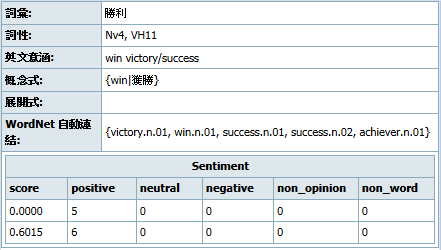
\includegraphics[scale=0.55,center]{e-hownet.png}
            \end{figure}
        \end{frame}

\section{Demonstrative Experiment}
    \begin{frame}{\secname}
        \begin{itemize}
            \item Dataset: ANTUSD $\cap$ E-hownet, a total 12995 words
            \item Three sentiment analysis tasks
                \begin{itemize}
                    \item Opinion extraction: identify opinion words (\{\textbf{POS},\textbf{NEG}\}\ v.s. \textbf{NONOP})
                    \item Polarity classification: classify opinion words (\textbf{POS} v.s. \textbf{NEG})
                    \item Combined tasks (\textbf{POS}, \textbf{NEG}, \textbf{NONOP})
                    \begin{itemize}
                        \item $P=\frac{correct(opinion) \cap correct(polarity)}{proposed(opinioopinionn)}$
                        \item $R=\frac{correct(opinion) \cap correct(polarity)}{gold(opinioopinionn)}$
                        \item $F-score = \frac{2PR}{P+R}$
                    \end{itemize}

                    % \begin{equation}
                    % \begin{array}{l}
                    %     P=\frac{correct(opinion) \cap correct(polarity)}{proposed(opinioopinionn)}\\
                    %     R=\frac{correct(opinion) \cap correct(polarity)}{gold(opinioopinionn)}\\
                    %     F-score = \frac{2PR}{P+R}\\
                    % \end{array} 
                    % \label{eq:f-score}
                    % \end{equation}
                \end{itemize}
            \item Classifier: support vector machine (SVM) with linear kernel
        \end{itemize}
    \end{frame}
    \subsection{Preprocessing}
        \begin{frame}{\subsecname}
            \begin{itemize}
                \item Extract single label for each word
                \begin{enumerate}
                    \item \textbf{NOT}: Count(Not)$>$0
                    \item \textbf{NONOP}: Count(Non)$>$0  
                    \item \textbf{POS}: Count(Pos)$>$0 and Count(Neg)=0  
                    \item \textbf{NEG}: Count(Neg)$>$0 and Count(Pos)=0  
                    \item \textbf{NEU}: Count(Pos)=0, Count(Neg)=0 and Count(Neu)$>$0  
                \end{enumerate}
                \item Neutral words are dropped since there are only 16 of them
                \item Words not labeled are also dropped (e.g., Count(Pos)$>$0 and Count(Neg)$>$0)
            \end{itemize}    
        \end{frame}
    \subsection{Features}
        \begin{frame}{\subsecname}
            \begin{itemize}
                \item CopeOpi score in ANTUSD
                \item Synonym-Set index (SSI)
                    \begin{itemize}
                        \item Concept frame index of a word
                        \item Each word might belong to many concepts
                        \item Represented as a binary vector % each dimension corresponds to a concept
                    \end{itemize}
                \item Trained word embedding with the corpus LDC2009T14 (Chinese news)
                    \begin{itemize}
                        \item Word vectors % low coverage, high quality
                        \item Summation of char vectors % high coverage, low quality   
                    \end{itemize}
            \end{itemize}
        \end{frame}
    \subsection[allowframebreaks]{Results}
        \begin{frame}{Opinion Extraction}
            \begin{columns}
                \begin{column}[T]{.5\textwidth}
                    \begin{itemize}
                        \item COP, SSI has lower precision
                            \begin{itemize}
                                \item opinion extraction  is more semantic-oriented
                                \item Many words contain single SSI
                            \end{itemize}
                        \item Character vectors lead to less precise semantic representation
                        \item Features are complemented; combined features leads to improvement
                    \end{itemize}
                \end{column}
                \begin{column}[T]{.6\textwidth}
                    \begin{table}
                    \small
                    \centering
                    \tabcolsep=0.1cm
                    \begin{tabular}{cccc}
                    \hline
                    Feature(s) & Precision & Recall & f-score \\ \hline
                    COP        & 0.686     & 1.000  & 0.814   \\ \hline
                    SSI        & 0.693     & 0.993  & 0.816   \\ \hline
                    WV         & 0.784     & 0.936  & 0.854   \\ \hline
                    CV         & 0.765     & 0.919  & 0.835   \\ \hline
                    COP+SSI    & 0.740     & 0.914  & 0.818   \\ \hline
                    COP+WV     & 0.785     & 0.933  & 0.853   \\ \hline
                    COP+CV     & 0.764     & 0.917  & 0.833   \\ \hline
                    SSI+WV     & 0.789     & 0.937  & 0.856   \\ \hline
                    SSI+CV     & 0.772     & 0.920  & 0.840   \\ \hline
                    WV+CV      & 0.808     & 0.921  & 0.861   \\ \hline
                    \end{tabular}
                    \end{table}
                \end{column}
            \end{columns}
        \end{frame}
        \begin{frame}{Polarity Classification}
            \begin{columns}
                \begin{column}[T]{.5\textwidth}
                    \begin{itemize}
                        \item COP leads to a significant better result, reflecting is sentiment-oriented nature
                        \item Combining COP \& other features still leads to improvement
                        \item Combining word vectors and SSI also leads to improvement % which meancs SSI can be used to increas the quality of word embedding
                    \end{itemize}
                \end{column}
                \begin{column}[T]{.6\textwidth}
                    \begin{table}
                    \small
                    \centering
                    \tabcolsep=0.1cm
                    \begin{tabular}{cccc}
                    \hline
                    Feature(s) & POS f1 & NEG f1 & Average f1 \\ \hline
                    COP        & 0.973  & 0.976  & 0.974      \\ \hline
                    SSI        & 0.792  & 0.842  & 0.817      \\ \hline
                    WV         & 0.870  & 0.895  & 0.882      \\ \hline
                    CV         & 0.829  & 0.851  & 0.840      \\ \hline
                    COP+SSI    & 0.979  & 0.982  & 0.980      \\ \hline
                    COP+WV     & 0.981  & 0.984  & 0.982      \\ \hline
                    COP+CV     & 0.967  & 0.972  & 0.970      \\ \hline
                    SSI+WV     & 0.898  & 0.915  & 0.907      \\ \hline
                    SSI+CV     & 0.868  & 0.886  & 0.877      \\ \hline
                    WV+CV      & 0.899  & 0.916  & 0.908      \\ \hline
                    \end{tabular}
                    \end{table}
                \end{column}
            \end{columns}
        \end{frame}
        \begin{frame}{Combined Task}
            \begin{columns}
                \begin{column}[T]{.5\textwidth}
                    \begin{itemize}
                        \item COP outperforms the others
                        \item Both the numerator of precision and recall are affected by COP’s better polarity classification ability
                        \item Only the denominator is affected by COP's worse opinion  extraction  ability
                        \item WV+CV outperforms WV due to coverage issue
                    \end{itemize}
                \end{column}
                \begin{column}[T]{.6\textwidth}
                    \begin{table}
                    \small
                    \centering
                    \tabcolsep=0.1cm
                    \begin{tabular}{cccc}
                    \hline
                    Feature(s) & Precision & Recall & f-score \\ \hline
                    COP        & 0.912     & 0.927  & 0.920   \\ \hline
                    SSI        & 0.706     & 0.679  & 0.692   \\ \hline
                    WV         & 0.737     & 0.767  & 0.752   \\ \hline
                    CV         & 0.689     & 0.721  & 0.705   \\ \hline
                    COP+SSI    & 0.864     & 0.945  & 0.903   \\ \hline
                    COP+WV     & 0.850     & 0.902  & 0.875   \\ \hline
                    COP+CV     & 0.840     & 0.869  & 0.854   \\ \hline
                    SSI+WV     & 0.764     & 0.796  & 0.779   \\ \hline
                    SSI+CV     & 0.732     & 0.755  & 0.743   \\ \hline
                    WV+CV      & 0.764     & 0.813  & 0.787   \\ \hline
                    \end{tabular}
                    \end{table}
                \end{column}
            \end{columns}
        \end{frame}

\section{Conclusion}
    \begin{frame}{\secname}
        \begin{itemize}
            \item A so far the largest Chinese sentiment dictionary
            \item Manually sentiment labels \& machine estimated sentiment scores 
            \item Three experiments were conducted to demonstrate the usage of ANTUSD
        \end{itemize}
    \end{frame}

    \begin{frame}{}
        \begin{center}
            \huge
            Q \& A
        \end{center}
    \end{frame}

\end{document}
